


\documentclass[conference]{Iris_detect}

\usepackage{graphicx}
\graphicspath{ {./images/} }

\usepackage[rightcaption]{sidecap}

\usepackage{wrapfig}
\ifCLASSINFOpdf
\else
\fi



\begin{document}
\title{Biometric Identification using Iris Recognition}

\author{Balram Choudhary$(16116015)$ and Varun Rathore$(16116074)$\\ Indian Institute of Technology,\\Roorkee 
}
\maketitle
\begin{abstract}
Iris recognition has become a popular research topic in recent years.Due to its high reliability and nearly zero error in recognition rates, it has come in high demand in security areas. Its application include border safety and control in airports, harbors, controlling authorized entrance in laboratory which requires high security , identification for Automatic Teller Machine, can be used as locker for preserving values, a secure lock for areas where authorization is limited to few person like police evidence room, presidential safe room and other super secure places where entry is restricted. There are mainly three stages of iris recognition system :image acquisition and preprocessing, feature extraction and template matching. A literate review of the most prominent algorithm implemented is presented.
\end{abstract}
\IEEEpeerreviewmaketitle



\section{Introduction}
Electronic arena is witnessing rapid sophisticated , a large and important change. Recognition has become a role of large and effective especially after the advancement of information technology.
A term "Biometric" indicates to identification and authentication of an individual identity based on unique features or characteristics in individual.\cite{Biometric}
The best biometric which can be used for recognition should have following traits
\begin{itemize}
    \item Universal : Each and every person should have specific biometric trait. It should be universally available to all human beings
    \item Unique : The trait acquired by person should be sufficiently different in terms of characteristic
    \item Collectible : Biometric trait should be collect able so make comparison for recognition using that trait
    \item Permanent Trait must not change with time allowing for repeatable measures otherwise there will be no use of it.
\end{itemize}
Every biometric system is made up of following building blocks
\begin{itemize}
    \item Sensor : A sensor that responds to biological stimulus  to generate signal that can be measured or interpreted.
    \item Feature Extraction Algorithm : It  detects and isolates portions of digital signal emanated out of a sensor which contains identifying properties .The algorithm creates descriptors or characteristic features per signal
    \item Searching Algorithm :A search and Compare algorithm takes an input characteristic feature and compares it with stored feature(s) and output  either success or failure of the outcome.
    \item  Database–An Database is collection of templates on which a given search & match algorithm operates. 
\end{itemize}
Biometric recognition system  might include fingerprints, retina pattern, iris , hand geometry,vein patterns,voice password,or signature dynamics.
Iris recognition is biometric used for purpose of identification and security.It is annular portion between dark pupil and white sclera.It has rich texture information which is used for biometric recognition system.
Iris recognition system is in high demand because its error rate is extremely low. It is permanent biometric i.e it remains stable through out life. It is also genetic independent i.e. no two eyes are same.Iris recognition is also great for security purposes because it does not change with age , expression, posture.
One of most challenging and crucial step in iris recognition system is iris segmentation.The circular Hough transform is used to detect iris and pupil, . Before applying transform, preprocessing steps involving morphology and filtering takes place to remove noise. Then using canny edge detector, outline of eye image. The edge image is then transformed to parameter or Hough space for a range of radii in order to determine the center and radius of pupil and iris.There are various factor which need to be consider before analyzing iris for recognition. There is stretching due to variation in pupil diameter  and offset due to lack of cocentricity. Implementation of recognition system requires conversion from cartesian coordinate system to normalised polar coordinate system using Daugman's transformation.
\section{Methodology}
Iris detection system can be implemented under following sub headings:
\begin{itemize}
    \item Image Acquisition
    \item Image Preprocessing
    \item Feature Extraction
    \item Template Matching
    \item Result
\end{itemize}


\subsection{Image Acquisition}
Image Database is taken from MMU database\cite{MMU}.It
comprises of 450 images, captured by a semi automated camera dedicated for iris capturing (LG Iris Access 2200) at 7-25 cm distance range. The images in MMU database have been collected from 100 volunteers of different ages and nationalities, with each volunteer contributing 5 images from each eye. The iris images in MMU database are homogeneous, and have been taken using an NIR light source at a close distance with human subject cooperation, introducing eyelashes obstruction and eye rotation  
\subsection{Image Preprocessing}
Image Processing is divided into further steps
\begin{itemize}
    \item Pupil Boundary Extraction 
    \item Iris Boundary Extraction
    \item Iris Normalization
    \item Iris Image enhancement
\end{itemize}
\subsubsection{Image Imcomplement}First the image complement is analyzed. Areas  of  dark pixels surrounded by lighter pixels were replaced by the lighter pixels. The image is inverted using imcomplement function.In the output image, dark areas become lighter and light areas become darker.

\begin{figure}
\centering
   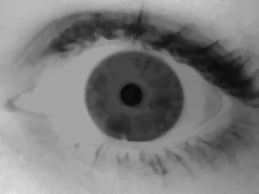
\includegraphics{Images/morph_operation_screenshot.png}
\caption{Result of Morphological Operation}
\end{figure}
 



\subsubsection{Illumination Removing} Removal of illumination that appears at centre of pupil is done by flood fill method.

\subsubsection{Pupil Segmentation}Pupil is a large region of homogeneous dark intensities with low variation due to coming lighting.For detecting 
\begin{itemize}
\item \textbf{Histogram Generation and Threshold Determination :}Generally iris images are captured under different illumination settings.Gray level(threshold) has to be found out such that 
    \begin{equation}
       b(x,y) = \left\{
       \begin{array}
         &1;   I(x,y) > T \\
         0;    I(x,y) <= T \\
       \end{array}
       \right.
    \end{equation}
    An iterative histogram based thresholding method with averaging filter is applied.Enrichment median filter is used on raw eye image to eliminate noise and to support clustering in pixel histogram.The outcome of histogram is to find a point that can be used to threshold the image. 
    Gray scales in histogram of an eye image generally consist of three regions: lower, medium and high. Lower region generally comprises gray levels that correspond to pupil and eyelashes. Gray level to medium correspond to iris and eyelids and High region corresponds to sclera and other part of eye. 
\item \textbf{Image Binarisation and Removal of noise}Image is binarised based on threshold value Eye Image sometimes have some cases where lashes is as dark as pupil which will appear in resulting binarised image hence act as a barrier in detection of pupil.Hence eyelashes can be removed by median filtration

\begin{itemize}
Median Filtration :It is semi low pass filter that helps in removing unwanted pixels without manipulating edges pixel.The values of pixel in window are sorted and median value is chosen. 
\end{itemize}
\item\textbf{Connected Component and Radius Calculation :} Connected Component algorithm is used to detect pupil from image. The algorithm basically extract different region which is a set of pixel with similar intensity and neighbours to each other. Region are then labelled .
coordinate of Circle thus labelled is calculated by finding centroid of figure Raduis of circle is distance between centre point and farthest point on the edge thus marked.
\begin{figure}
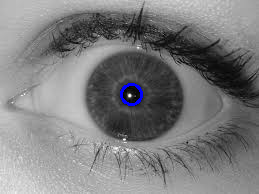
\includegraphics{Images/pupil_screenshot.png}
\caption{Result of Pupil detection}
\end{figure}
    \begin{figure}

\includegraphics{Images/canny_screenshot.png}
\caption{Result of canny edge detection}
\end{figure}



 
\end{itemize}
\subsubsection{Iris Boundary Extraction and Segmentation}
The important step of iris recognition is to isolate the actual iris region in a digital eye image.This step detects the inner and outer boundaries of iris.\cite{iris} It is not mandatory that centre of iris and centre of of pupil coincide with each other.It is important steps as correct boundary region  is needed to generate template for efficient matching. There are several algorithm for iris boundary extraction like Integro-Differential operator, Hough Transform, Discrete Circular Active Contour, Bisection method and Black hole search method. This step is implemented using Hough Transform method
\begin{itemize}
    \item \textbf{Convert Image into Gray Scale :}This step convert original image into Gray Scale
    \item \textbf{Edge Detection:}This steps generate edge map of object within images.The method used here is canny edge detection.
    The algorithm runs in 5 steps
    \begin{itemize}
    \item \textbf{Smoothing : }$Median filtering$ is used to remove noise.It computes median of all pixels under the kernel window and central pixel is replaced with its median value. This is effective method in removing salt and pepper noise. Unlike other filtering method , central element if always replaced by some pixel value in image,hence reduces noise effectively.
    \item \textbf{Computing Gradients :} The edge are marked where gradients of image has maximum magnitude.
    \begin{equation}
    D=\sqrt{D_{x}(x,y)^2 +D_{y}(x,y)^2}
    \end{equation}
    \begin{equation}
    \theta = arctan(D_{x}(x,y)/D_{y}(x,y))
    \end{equation}
    \item \textbf{Non-maximum suppression : } This step only keeps those pixels on an edge with highest gradient magnitude.
    \item \textbf{Double thresholding :} Potential edges are computed by this method.
    \item \textbf{Edge tracking by hysteresis :}Finally edges which are not connected to any edge are neglected and true edges are determined.
    \end{itemize}
    
    \item \textbf{Hough Transform:}Hough Transform is a standard computer vision algorithm that can be used to detect shapes which can be expressed in parametric form such as line, hyperbola, parabola and circle. Circular Hough Transform is used to detect circles of fixed radii in an image. General equation of circle with radius $r$ and centre $(a,b)$ can be expressed as 
    \begin{equation}
    r^2 =(x-a)^2 +(y-b)^2
    \end{equation}
    Its parametric co-ordinates are
    \begin{equation}
    x=a+r*cos(\theta)
    \end{equation}
    \begin{equation}
    y=b+r*sin(\theta)
    \end{equation}
    The voting procedure is implemented using hough transform in order to detect desired contour from edge map.it is computed by drawing circle at every point in edge image. For every point where the perimeter of a drawn circle passes,it cast a vote in hough space.The center coordinate and radius of circle with maximum votes is defined as contour of interest.\\
    Its main advantages are its insensitivity to noise and its capability to extract even in areas with pixel absence.
    \begin{figure}
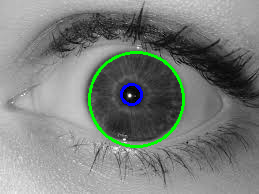
\includegraphics{Images/houghman_method_screenshot.png}
\caption{Result of Hough Transform}
\end{figure}
    \item \textbf{Daugman’s Integro-differential Operator:}This method make use of integro-differential operator \cite{daugman}for locating circular iris and pupil regions,it can also detect arcs of upper and lower eyelids. The operator is expressed in following way
    \begin{equation}
    max_{r^{'},x_{\rho},y_{\sigma}}|G_{\sigma}(r)*∂/∂r∫_{r,x_{0},y_{0}}I(x,y)/2\pi*r ds|
   \end{equation}
   where I(x,y) is eye image, r is the radius to search for, $G_{\sigma}(r)$ is a Gaussian smoothing function and s is contour of circle given by r, $x_{0}$,$y_{0}$. By varying the radius and centre x and y position of circular contour, the operator searches for path where there is maximum change in pixel values. The operator is applied iteratively with amount of smoothing progressively reduced in order to attain precise localization. Eyelids are localized in similar manner.
   This method can be seen as a variation of Hough Transform, since both methods make use of first derivative of image and perform search operation to find geometric parameters.Since it works with raw derivative , it does not suffer from thresholding. However, algorithm fails when there is noise in image.
\end{itemize}
\begin{figure}
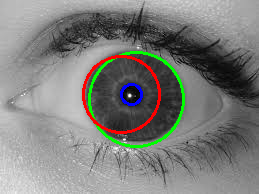
\includegraphics{Images/daugman_method_screenshot.png}
\caption{Result Daugman's Integro Differential Operator(red) along with hough transform(green)}
\end{figure}
\subsubsection{Iris Normalization :}
Images of same iris can be captured in different spatial condition and illumination variation which may change size of pupil and hence will result in deformation of iris texture.Hence region has to be normalized to compensate these changes.Normalization is a process the changes range of pixel intensity values. It will produce iris regions which have the same constant dimension. It has advantage that two images of iris under different condition will have same characteristic feature at same same location.
\begin{itemize}
\textbf{Daugman’s Rubber Sheet Model : }Daugman suggested normal Cartesian to polar transformation so as to map each pixel in iris area into a pair of polar coordinates $(r,\theta)$ where $r$ and $(\theta)$ are on the interval $[0,1]$ and $[0,2\pi]$. It can be expressed as\\\\

\begin{equation}
    
I(x(r,\theta),y(r,\theta))\rightarrow I(r,\theta)
\end{equation}
\\\\
such that\\
\begin{equation}
x(r,\theta)=(1-r)x_{p}(\theta) +rx(\theta)
\end{equation}
\begin{equation}
y(r,\theta)=(1-r)y_{p}(\theta)+ry(\theta)
\end{equation}
where \\\\
\begin{expression}
 I(x,y), (x,y), (r, \theta), (x_{p}, y_{p}), (x_{i}, y_{i}) 
\end{expression} 
\begin{figure}

\includegraphics{Images/normalise_image_screenshot.png}
\caption{An example of Normalisation of image}
\end{figure}

\\\\represent the iris region, Cartesian coordinates, polar coordinates, coordinates of the pupil and iris boundaries along θ direction respectively. 
The non concentric polar representation is normalized to a fixed size rectangular block. It can compensate non concentric pupil displacement, imaging distance, pupil dilation.It does not compensate for rotational
inconsistencies. In the Daugman system, rotation is compensated  during matching by shifting the iris images in the θ direction until two iris images are aligned.
\textbf{\\Implementation of Daugman Rubber Sheet Model:}
Daugman's rubber sheet model \cite{daugman2}is implemented for normalization of iris regions.As a reference point, pupil centre is chosen and radial vectors pass through the iris region.Some points are selected randomly along each radial line and this is defined as radial resolution. The number of lines around iris in angular region is defined as angular resolution. Since it is not necessary that pupil and iris are not concentric , a remapping formula is needed to re scale points depending on angular position  around circle. This can be expressed as
\begin{equation}
    r^{'}=\sqrt{\alpha\beta}+^{-}\sqrt{\alpha\beta^2 -\alpha -r_{s}^2}
\end{equation}
with 
\begin{equation}
\alpha =\sigma^2_{x}+\sigma^2_{y}
\beta=cos(\pi- arctan(\sigma_y/\sigma_x)-\theta)

\end{equation}
where displacement of centre of pupil with respect to centre of iris is given by \sigma_{x},\sigma_{y} and \ $r^{'}$ is distance between edge of pupil and iris edge at an angle, \theta $ \around the region, and $r_{l}$ \is radius of iris.function first gives radius of iris as function of  $\ \theta.$
Number of points which are chosen along radial line are constant so as to take a constant number of radial points irrespective of how narrow or wide radius is at particular angle. The pattern is created by backtracking which helps to find Cartesian coordinated of data points from radial and angular position in pattern. Normalization produces a @D array with horizontal dimensions of angular resolution and vertical dimension of radial resolution from 'doughnut region'. An other array of 2 dimension is created for marking reflections,eyelashes and eyelids detected in segmentation stage.  In order to prevent corruption of normalized pattern from non-iris data, data points are discarded which occur along the border of pupil or iris.In this method, rotational inconsistencies are removed at matching stage.$ 
\\
\section{Conclusion}
We have successfully implemented pupil detection using Histogram generation and threshold detection and result is shown in figure2. Further, Iris segmentation is performed successfully using Hough Transform and Doughman integro-differential operator and result  of these method are shown in figure 4 and figure 5 respectively.Further for normalization of image from Cartesian coordinate to polar coordinate system Doughman Rubber sheet model is applied which will be later used for feature extraction and matching. The normalized image is shown in figure 5.


\section*{Acknowledgment}


The authors would like to thank Prof. Saumik Bhattacharya for giving us this opportunity to implement iris recognition system.




\begin{thebibliography}{1}
\bibitem{Biometric}
S. Sanderson, J. Erbetta. Authentication for secure environments based on iris
scanning technology. IEE Colloquium on Visual Biometrics, 2000.

\bibitem{MMU}
Multimedia-University. MMU Database [Online].Available:http://pesona.mmu.edu.my/~cct
eo/. Last Accessed 
(Dec 2016).

\bibitem{Daugman}
Daugman,J.2004.How iris recognition works . IEEE Trans , CSVT 14 , 21 — 30 
\bibitem{Daugman2}
Daugman,J.The importance of being random : Statistical principles of iris recognition . Pattern Recognition , vol. 36 , num.2 , pp.279-291,2003 

\bibitem{iris}
A.Poursaberi,B.N.Araabi,"ANovel Iris Recognition System Using Morphological Edge Detector and Wave l e t Phase Features",ICGST International Jour nalon Graphics ,Vision and Image Processing ,P1150517004,June2005
\end{thebibliography}



\end{document}


